\documentclass{article}
\usepackage{graphicx}
\usepackage{natbib}
\usepackage{graphicx}
\bibliographystyle{plainnat}
\usepackage{fancyheadings}
\usepackage{tabularx}
\usepackage{alltt, parskip, boxedminipage}
\usepackage{makeidx, multirow, longtable, tocbibind, amssymb}
%\usepackage{fullpage}
\makeindex
\usepackage[usenames]{color}
\definecolor{darkblue}{rgb}{0,0.05,0.35}

\usepackage[dvips, pagebackref, pdftitle={}, pdfcreator={epydoc 2.1}, bookmarks=true, bookmarksopen=false, pdfpagemode=UseOutlines, colorlinks=true, linkcolor=black, anchorcolor=black, citecolor=black, filecolor=black, menucolor=black, pagecolor=black, urlcolor=darkblue]{hyperref}
\setlength{\textheight}{21.5cm}
\setlength{\textwidth}{18cm}
\setlength{\hoffset}{-3.0cm}
\setlength{\footskip}{1.5cm}
\setlength{\headsep}{2.5cm}
\setlength{\voffset}{-2.5cm}
\newlength{\BCL} % base class length, for base trees.

\usepackage{everyshi}
 \makeatletter
 \let\totalpages\relax
 \newcounter{mypage}
 \EveryShipout{\stepcounter{mypage}}
 \AtEndDocument{\clearpage
    \immediate\write\@auxout{%
     \string\gdef\string\totalpages{\themypage}}}
 \makeatother

\newcommand{\esofooter}{

\includegraphics[height=1cm]{durlogo.eps}
{\bf \large Centre for \AA dvanced Instrumentation}
}
\newcommand{\esoheaderl}{

\includegraphics[height=1cm]{durlogo.eps}
\begin{tabularx}{9cm}{c}
\Large {\bf \esotitle} \\ \large {\bf(\esodoctype)}\\
\rightmark\hspace{0.1cm}
\end{tabularx}
\vfill
}
\newcommand{\esoheaderc}{
}
\newcommand{\esoheaderr}{
\begin{tabular}{|l|l|}\hline
Doc. number: & \esodocno \\ \hline
Release date: & \esoreleasedate \\ \hline
Issue number: & \esoissue \\ \hline
Page number: & Page \thepage \ of \totalpages \\ \hline
Author(s) & \esoauthorname \\ \hline
\end{tabular}


}

\pagestyle{fancy}
\cfoot[]{}
\lfoot[\esofooter]{\esofooter}
\lhead[\esoheaderl]{\esoheaderl}
\chead[\esoheaderc]{\esoheaderc}
\rhead[\esoheaderr]{\esoheaderr}
\renewcommand{\sectionmark}[1]{\markboth{#1}{#1}}

\newenvironment{Ventry}[1]%
  {\begin{list}{}{%
    \renewcommand{\makelabel}[1]{\texttt{##1:}\hfil}%
    \settowidth{\labelwidth}{\texttt{#1:}}%
    \setlength{\leftmargin}{\labelsep}%
    \addtolength{\leftmargin}{\labelwidth}}}%
  {\end{list}}


\begin{document}
\newcommand{\daspproject}{AO Simulation Project}
\newcommand{\dasptitle}{AO Simulation parameter GUI}
\newcommand{\daspdocno}{AOSIM-PAR-UoD-001}
\newcommand{\daspdoctype}{Internal}
\newcommand{\daspissue}{0.1.1}
\newcommand{\daspreleasedate}{\today}
\newcommand{\daspauthorname}{Alastair Basden}
\newcommand{\daspauthortype}{AO sim team member}
\newcommand{\daspapprovername}{Alastair Basden}
\newcommand{\daspapprovertype}{AO sim team member}
\newcommand{\daspreleasername}{Alastair Basden}
\newcommand{\daspreleasertype}{AO sim team member}
\newcommand{\daspreviewername}{Alastair Basden}
\newcommand{\daspreviewertype}{AO sim team member}
\newcommand{\daspchangerecord}{
\begin{tabular}{|l|l|l|l|}
\hline
Issue number & Release date & section(s) affected & Description of
change/remarks\\ \hline
0.1.0 & 051111 & All & First draft \\ \hline
0.1.1 & 051111 & All & Corrections made to first draft\\ \hline
\end{tabular}
}
\newcommand{\daspnotificationlist}{
Alastair Basden\\
Francois Assemat\\
Richard Wilson\\
Tim Morris\\
Tim Butterley\\
Ali Bharmal\\
}
\newcommand{\daspabbreviations}{
\begin{tabular}{rl}
AO & Adaptive Optics\\
ESO & European Southern Observatory\\
\end{tabular}
}
\newcommand{\daspapplicabledocs}{
\begin{tabular}{|l|l|l|}\hline
AD Number & Document title & Doc number/publication/location \\ \hline
AD01 & Simulation API document & AOSIM-API-UoD-001\\ \hline
AD02 & Simulation for dummies document & AOSIM-DUM-UoD-001\\ \hline
\end{tabular}
}
\newcommand{\dasprefdocs}{
\begin{tabular}{|l|l|l|}\hline
RD number & Document title & Doc number/publication/location \\ \hline
RD01 & Durham FPGA website & www.durham.ac.uk/rtcs.project \\ \hline
\end{tabular}
}
\title{\dasptitle}



\thispagestyle{empty}
%This next command provides the CVS tag.  If you want a cvs tag on
%your document, add the following line at the start of the document,
%after replacing the & signs with dollar signs...
%\newcommand{\cvsID}{& &Id& (CVS)&}
\providecommand{\cvsID}{CVS ID not provided: document made on \today}

\begin{center}

\includegraphics{durlogo.eps}
\end{center}
\vspace{0.5cm}
\Huge
\begin{center}
\esoproject\\
\end{center}
\Large
\vspace{1cm}


{\bf 
\begin{tabular}{ll}
Document title: & \esotitle \vspace{0.5cm}\\ 

Documentation number: & \esodocno \vspace{0.5cm}\\ 

Document type: & \esodoctype \vspace{0.5cm}\\ 

Issue number:& \esoissue \vspace{0.5cm}\\ 

Release date: & \esoreleasedate \\ 

\end{tabular}
}

\normalsize
\vfill

\begin{tabular}{|l|l|l|p{5cm}|}
\hline
Document & \esoauthorname & Signature &\\
prepared by & \esoauthortype & and date &\\ \hline
Document & \esoapprovername & Signature &\\
approved by & \esoapprovertype & and date &\\ \hline
Document & \esoreleasername & Signature &\\
released by & \esoreleasertype & and date &\\ \hline
Document & \esoreviewername & Signature &\\
reviewed by & \esoreviewertype & and date &\\ \hline
\end{tabular}

\small
%\begin{alltt}
\cvsID
%\end{alltt}
\normalsize
%\lfoot[\esofooter]{\esofooter}
%\lhead[\esoheaderl]{\esoheaderl}
%\chead[\esoheaderc]{\esoheaderc}
%\rhead[\esoheaderr]{\esoheaderr}
%\renewcommand{\sectionmark}[1]{\markboth{#1}{#1}}

\pagebreak



\begin{center}
\Large
{\bf Change record\\ \vspace{1cm}}
\normalsize
\esochangerecord
\end{center}
\vspace{2cm}

\begin{center}
\Large
{\bf Notification list\\ \vspace{1cm}}
\normalsize
\esonotificationlist
\end{center}

\pagebreak

\begin{center}
\Large
{\bf Acronyms and abbreviations\\ \vspace{1cm}}
\normalsize
\esoabbreviations
\end{center}

\pagebreak

\begin{center}
\Large
{\bf Applicable documents\\ \vspace{1cm}}
\normalsize

\esoapplicabledocs
\end{center}
\vspace{2cm}

\begin{center}
\Large
{\bf Reference documents \\ \vspace{1cm}}
\normalsize

\esorefdocs
\end{center}

\pagebreak
\tableofcontents
\pagebreak

\section{Introduction}
This guide is intended to provide information about the parameter
setup GUI (paramgui.py), part of the AO simulation package.  Further
information about the AO simulation package can be found in
\citet{overview}.

The parameter GUI is used to set the values of variables that the
simulation requires.  These values are written to an XML parameter
file, which can then be parsed by the simulation when it is started
(use the \texttt{--param-file=FILENAME} commandline switch when
running the simulation).  The parameter GUI is written in python using
GTK~2.0.  Details of the parameter GUI API are not given here, as it
is unlikely that a simulation programmer will need to alter the GUI.

\section{The paramgui GUI}
Fig.~\ref{fig:paramgui} shows the parameter GUI during use.  The
functionality of this GUI will now be described.
\begin{figure}
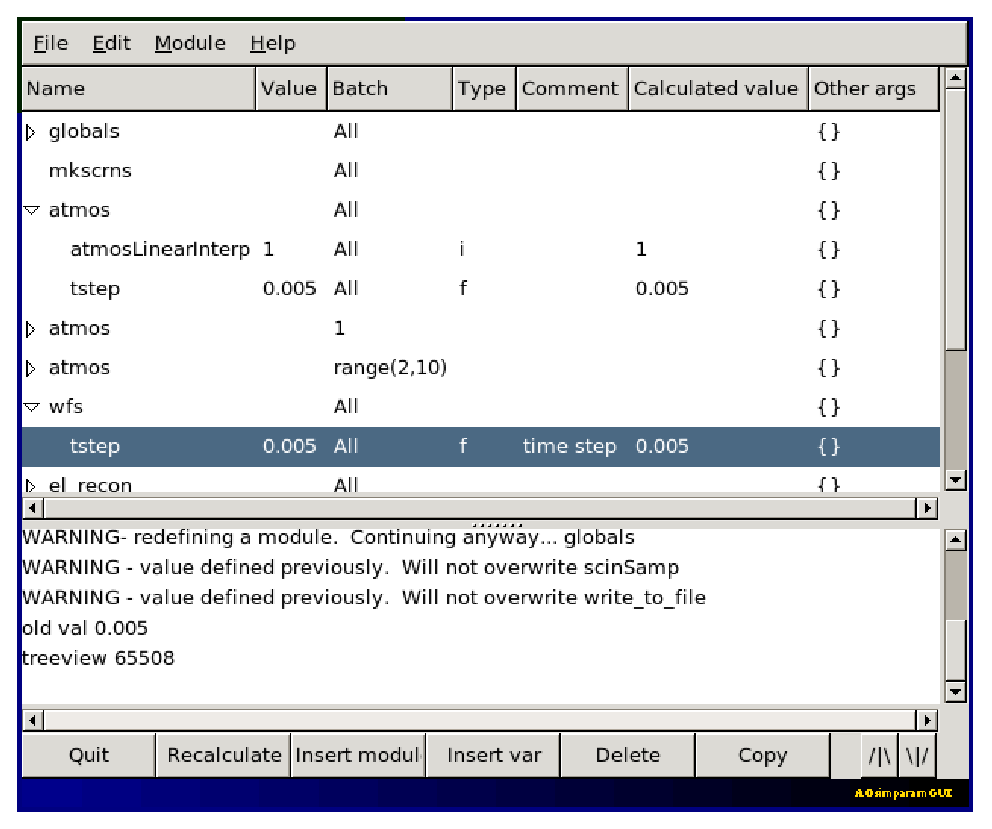
\includegraphics{pics/paramguimain.eps}
\caption{A screenshot of the parameter GUI during use.}
\label{fig:paramgui}
\end{figure}


\subsection{The main window}
As shown in Fig.~\ref{fig:paramgui}, the parameter GUI is divided into
several sections, namely a menu bar, a variable tree, a message
window, and a row of buttons.  

In the variable tree, the currently
defined variables and modules are displayed, along with all data that
will be written to an XML file.  The variables belonging to a module
can be shown or hidden by clicking on the small triangle at the left
edge of the tree.  Modules and variables can be edited by clicking on
them and typing in new values or other information.  The column
headings are as follows:
\begin{description}
\item[Name] The name of the module or variable.  Within the
  simulation, the module is selected automatically, depending on the
  current science module, and the variable can be selected using the
  \texttt{getVal(``Name'')} method.
\item[Value] For variables, this is the value that the variable should
  take.  The text inserted here will depend on the value inserted in
  the {\bf Type} column, and can include arbitrary Python code for
  certain types.
\item[Batch] Text representing the batch number (or numbers) for which
  the module or variable is valid.  This is useful if you wish to run
  a given simulation many times changing a parameter each time.  The
  text here can be ``All'', a Python list or integer.  
\item[Type] The type of the variable, which can be one of ``i'' (int),
  ``f'' (float), ``code'' (python code which is executed using exec),
  ``list'' (list), ``string'' (a string), among others.
\item[Comment] A comment, for the user to read.
\item[Calculated value] The value which would be returned by a call to
  \texttt{getVal(``name'')} after the parameter file has been parsed.
  This can be different from the {\bf Value} column if for example
  there is Python code in the {\bf Value} column.
\item[Other args] Other arguments in the parameter file, which as yet
  are not used in the simulation, but may be present for other reasons.
\end{description}

The message window typically contains
warning message if a mistake has been made, and other information
relevent for the user.

\subsection{The button bar}
\subsubsection{Quit}
The quit button will exit the paramgui program.  At present, no
checking (i.e.\ whether the current parameters have been saved) is
carried out, though this may be altered in the future.

\subsubsection{Recalculate}
The recalculate button is used to update the {\bf Calculated value}
column of the tree display, as this is not automatically updated when
a variable value is changed.  If there is an error, this will be
reported in the message window, and the user should then correct this.

\subsubsection{Insert module}
The insert module button allows the user to begin a new module.  This
is similar to pressing the insert key on the keyboard.

\subsubsection{Insert var}
The insert var button allows the user to insert a new variable either
after the currently selected variable, or at the start of the
currently selected module.  This is similar to pressing the insert key
on the keyboard.


\subsubsection{Delete}
\label{sect:deletebutton}
The delete button allows the user to delete a module or variable.  No
checking is performed, the module is deleted straight away.  This is
the same as pressing the delete key.

\subsubsection{Copy}
\label{sect:copybutton}
The copy button will copy a module or variable, creating an identical
copy immediately next to the existing one.

\subsubsection{Up}
The Up button will move a module up by one place.

\subsection{Down}
The Down button will move a module down by one place.

\subsection{Menus}
\subsubsection{The file menu}
The {\bf File} menu contains some of the standard items found in a file
menu, namely:
\begin{description}
\item[New] Start a new simulation parameter file (disposing of any
  existing parameters).
\item[Open] Open a simulation parameter file.
\item[Save] Save a simulation file.
\item[Save as] Save a simulation file with a new filename.
\item[Quit] Quit the GUI.
\end{description}

The {\bf Edit} menu contains only a ``copy'' item, which performs the same
task as the Copy button described in section~\ref{sect:copybutton}.

The {\bf Module} menu contains the following items:
\begin{description}
\item[Skeleton from simulation file] Presents the user with a file
  selection dialog, allowing the user to select a simulation Python
  file.  This file is then parsed for all the variables that it
  requires, and these are placed in a new module within the variable
  tree window.  This is a quick way for a user to build up a
  configuration file.
\item[Import from param file] Presents the user with a file selection
  dialog, allowing the user to select an existing parameter file.  The
  user is then presented with a list of modules within the file, as
  shown in Fig.~\ref{fig:paramguimodule}.  The user can then select
  one of these modules, which is imported into the current parameter
  file, and variable tree window.
\item[Delete] Delete a module from the current parameter file.  This
  has the same functionality as the Delete button described in
  section~\ref{sect:deletebutton}.  
\end{description}

\begin{figure}
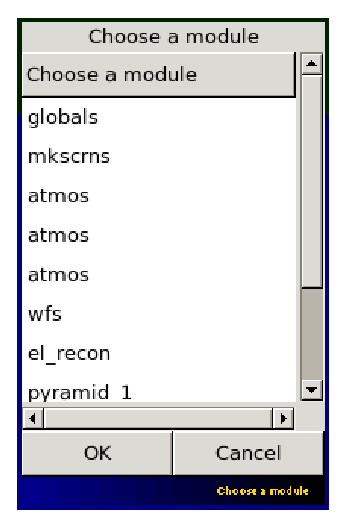
\includegraphics{pics/paramguimodule.eps}
\caption{A screenshot of the module selection widget displayed when
  the user is importing a module from an existing parameter file.}
\label{fig:paramguimodule}
\end{figure}

The {\bf help} menu currently contains only an ``about'' item which
prints a message into the message window.

\section{conclusion}
The parameter GUI has been described, and you should now be able to
use it.  

\bibliography{references}
\printindex
\end{document}
